\documentclass{article}

\usepackage{AcademicReportCn}

% enable Chinese
\usepackage[UTF8]{ctex}

% setting for levels
\usepackage{hyperref}
\setcounter{secnumdepth}{2}
\setcounter{tocdepth}{2}
\hypersetup{
    bookmarksopenlevel = 3,
    citecolor = red,
	colorlinks		=	true,
	bookmarks		=	true,
	bookmarksopen	=	true,
    % bookmarksdepth  =   2,
	pdfstartview	=	Fit,
	pdftitle		=	{画图建议指南},
	pdfauthor		=	{钟家鑫},
}

% biber is required to compile: xelatex -> biber -> xelatex*2
\usepackage[
    giveninits=true, 
    maxbibnames=99,
    % style=numeric,
    sorting=none,
    doi = false,
    url = false,
    isbn = false,
    style=ieee, citestyle=numeric-comp,
    ]{biblatex}
\addbibresource{biblatex.bib}

% open book mark at arbitrary level
\usepackage[open, numbered]{bookmark}
% opt: numbered --- show numbers in the bookmark

% for some dummy text
\usepackage{lipsum}

% see https://tex.stackexchange.com/questions/226481/appendix-section-title
\usepackage[title]{appendix}


\title{\textbf{画图建议指南}}
\author{钟家鑫}
\date{\today}

% \usepackage{mlmodern}


\begin{document}
\maketitle
% enable Page 1 of xx at the first page
\thispagestyle{firststyle}

\section{简介}
本文档总结论文画图的一些建议。

\section{二维图}
Figure~\ref{fig:39:f020390} shows the results of something.
\begin{figure}[!htb]
    \centering
    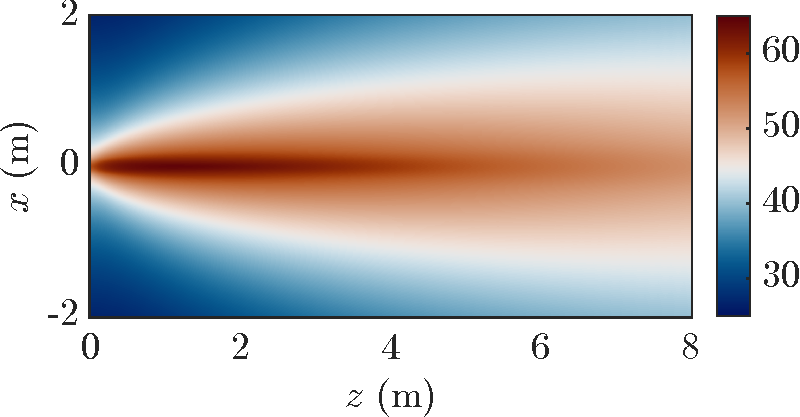
\includegraphics[width = 0.6\textwidth]{fig.pdf}
    \caption{二维图示例}
    \label{fig:2d_fig}
\end{figure}



\addcontentsline{toc}{section}{参考文献}
% https://tex.stackexchange.com/questions/261443/changing-bibliography-title-with-biblatex-within-the-document
\printbibliography[title=参考文献]

\end{document}


